\documentclass[12pt, reqno]{amsart}

%\usepackage{upgreek}
\usepackage[margin=3.5 cm]{geometry}
\usepackage{graphicx, mathabx}
\usepackage{color}
\usepackage{float}
%\usepackage{subfigure}
\newtheorem{theorem}{Theorem}[section]
\newtheorem*{theorem*}{Theorem}          %theorem without number
\newtheorem{prop}{Proposition}[section]
\newtheorem*{prop*}{Proposition}  % proposition without number
\newtheorem{coro}{Corollary}[section]
\newtheorem{lemma}[theorem]{Lemma}
\newtheorem{conj}{Conjecture}[section]
\newtheorem{obs}{Observation}[section]

\theoremstyle{definition}
\newtheorem{definition}[theorem]{Definition}
\newtheorem{example}[theorem]{Example}
\newtheorem{xca}[theorem]{Exercise}

\theoremstyle{remark}
\newtheorem{remark}[theorem]{Remark}

%\numberwithin{equation}

%    Absolute value notation
\newcommand{\abs}[1]{\lvert#1\rvert}
\newcommand{\norm}[1]{\lVert#1\rVert}
\DeclareMathOperator{\re}{Re}
\DeclareMathOperator{\im}{Im}
\newcommand{\ud}{\mathrm{d}}

\begin{document}

\title[Math 357 - Harmonic Analysis]{Problem set no. 4 - Isaac Vivivano}

\begin{titlepage}

\maketitle
I affirm that I have adhered to the Honor Code on this assignment.

Isaac  Viviano
   
\end{titlepage}

\section*{}


\section{Solutions:} 

\begin{itemize}

\vspace{0.2 cm}
\item {\bf{Problem 1 - Riemann-Lebesgue Lemma:}} 

\vspace{0.1 cm}
\begin{itemize}
\item[(a)] {\bf{Proof of Riemann-Lebesgue for continuous functions:}}

\begin{lemma}
For all $f\in\mathcal{T}$, if $N-1$ is the degree of $f$, for all $n\ge N$, \[
\vert \widehat{f}_n \vert = 0 
\]
\end{lemma}

\begin{proof}
   
Let $$f(t)=\sum_{k=-N}^{N}c_{k}e^{2\pi ikt}$$and let $\epsilon>0$ be given. 

\begin{align*}
\hat{f}_{n}&= \int_{0}^{1}\left(\sum_{k=-N}^{N}c_{k}e_{k}(t)\right)\overline{e_{n}(t)}\ dt\\
&= \int_{0}^{1}\sum_{k=-N}^{N}(c_{k}e_{k}(t)\overline{e_{n}(t)})\ dt\\
&= \sum_{k=-N}^{N}c_{k}\int_{0}^{1}e_{k}(t)\overline{e_{n}(t)}\ dt\\
&= \sum_{k=-N}^{N}c_{k}\cdot \delta_{n,k}\\
&= \begin{cases}c_{n} & \text{if } |n|\le N\\
0 & \text{if }|n|>N
\end{cases}
\end{align*}
Therefore, for all $n\ge N+1$ and $n\le -N-1$, $$|\hat{f}_{n}|=|0|=0$$
\end{proof}

\begin{prop}
For all $f\in\mathcal{C}(\mathbb{R;C})$, \[
\vert \widehat{f}_n \vert \to 0 ~\mbox{, as } \vert n \vert \to \infty ~\mbox{.}
\]
\end{prop}

\begin{proof}
   Let $f\in\mathcal{C}_{1}(\mathbb{R};\mathbb{C})$. Let $\epsilon>0$ be given. With the Weierstrass approximation theorem, pick $p\in \mathcal{T}$ such that $$\|f-p\|_{\infty}<\epsilon$$From Set 2, $$\left|[\widehat{f-p}]_{n}\right|\le\|f-p\|_{\infty}<\epsilon$$
And,
\begin{align*}
[\widehat{f-p}]_{n}&= \int_{0}^{1}(f(t)-p(t))\overline{e_{n}(t)}\ dt\\
&= \int_{0}^{1}f(t)\overline{e_{n}(t)}\ dt-\int_{0}^{1}p(t)\overline{e_{n}(t)}\ dt\\
&= 
\hat f_{n}-\hat p_{n}
\end{align*}
Let $N-1$ be the degree of $p$. Then, for all $|n|\ge N$,
\begin{align*}
\left|\hat{f}_{n}\right|&= |\hat f_{n}-\hat p_{n}+\hat p_{n}|\\
&\le \left|\hat f_{n}-\hat p_{n}\right|+\underbrace{|\hat p_{n}|}_{=0}\\
&= \left|[\widehat{f-p}]_{n}\right|\\
&<  \epsilon
\end{align*}
So, $$|\hat f_{n}|\rightarrow 0,\text{ as }|n|\rightarrow \infty$$
\end{proof}

\vspace{0.1 cm}
\item[(b)] {\bf{Proof of Riemann-Lebesgue for uniform limits of step functions:}}


\begin{itemize}
\item[(b-i)] 

Graph of $f=f_1+f_2+f_3$ defined by \begin{align}
f_1&= \frac{1}{2}\chi_{[0,\frac{1}{3})}\\
f_2&= \chi_{[\frac{1}{4},\frac{1}{2}]}\\
f_3&= \frac{3}{4}\chi_{[\frac{1}{2},\frac{3}{4}]}
\end{align}
\begin{figure}[H]
   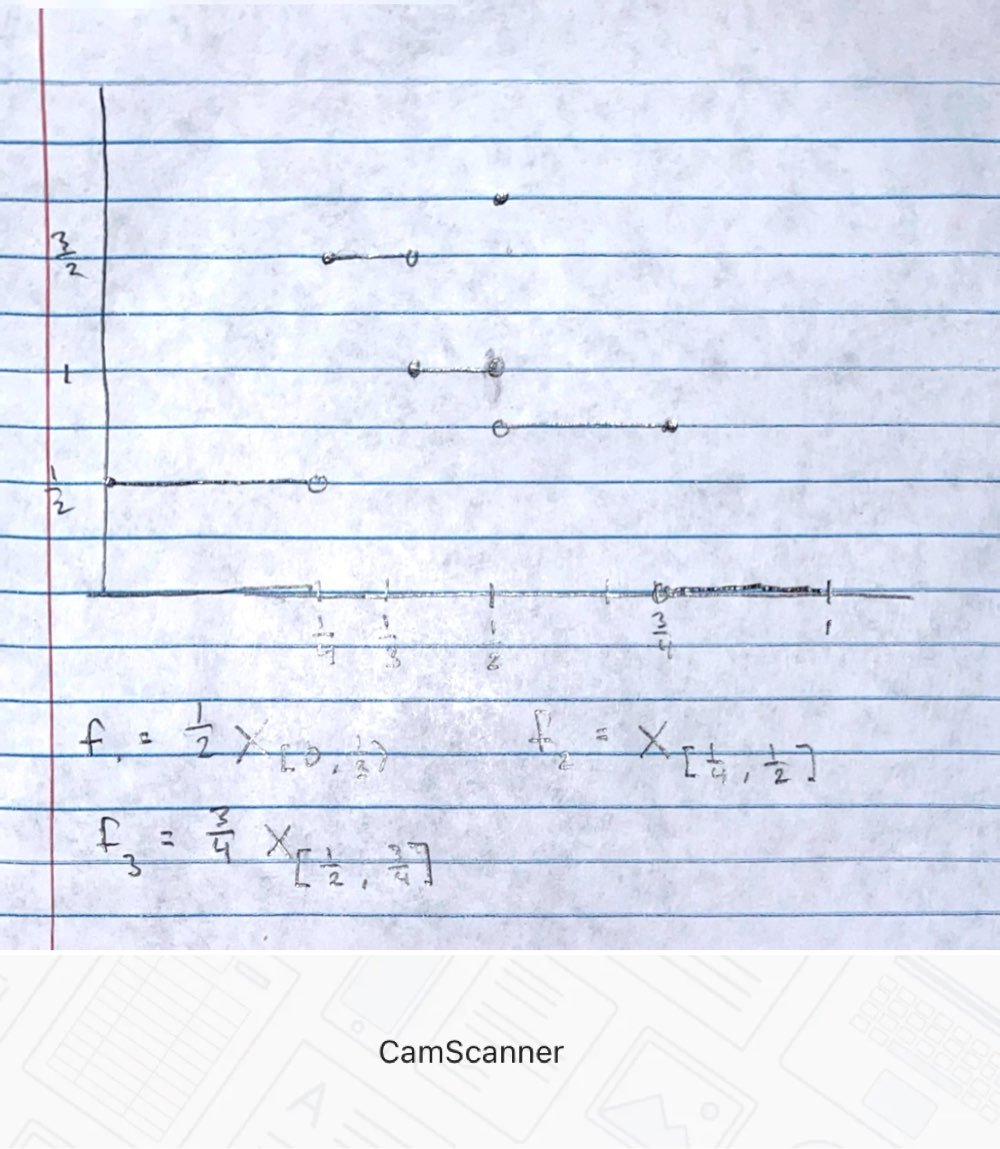
\includegraphics[width = 5in]{Long image 2024-03-04 21.40.22.jpg}
   
\end{figure}


\item[(b-ii)] 

\begin{lemma}
   For all 1-periodic step-functions $f$, \[\left|\hat f_n\right|\to0,\text{ as }|n|\to\infty\]
\end{lemma}

\begin{proof}

Let $c<d\in \mathbb{R}$ with $d-c<1$. Note that the Fourier coefficients of periodic extensions $\chi_{[c,d]}, \chi_{(c,d]},\chi_{[c,d)}$ are the same since changing the value of a Riemann integrable function at finitely many points does not change its integral. Define $f$ to be the 1-periodic extension of $\lambda\chi_{[c,d]}$ for some $\lambda\in \mathbb{C}$.

\begin{align*}
\left|\hat f_{n}\right|&= \left|\int_{0}^{1}f(t)\overline{e_{n}(t)}\ dt\right|\\
&\le \int_{0}^{1}|f(t)|\cdot\left|\overline{e_{n}(t)\ dt}\right|\ dt\\
&= \int_{0}^{1}|f(t)|\ dt
\end{align*}

\begin{align*}
\hat f_{n}&= \int_{0}^{1}f(t)\overline{e_{n}(t)}\ dt\\
&= \int_{c}^{c+1}f(t)\overline{e_{n}(t)}\ dt\\
&= \int_{c}^{d}\lambda e^{-2\pi int}\ dt\\
&= \frac{1}{2\pi in}\lambda e^{-2\pi int}\bigg|_{c}^{d}\\
&= \frac{\lambda}{{2\pi in}}(e^{-2\pi ind}-e^{-2\pi inc})\\
\left|\hat f_{n}\right|&= \left|\frac{\lambda}{{2\pi in}}(e^{-2\pi ind}-e^{-2\pi inc})\right|\\
&= \frac{|\lambda|}{{2\pi |n|}}\left|e^{-2\pi ind}-e^{-2\pi inc}\right|\\
&\le \frac{|\lambda|}{{2\pi |n|}}(\left|e^{-2\pi ind}\right|+\left|e^{-2\pi inc}\right|)\\
&= \frac{|\lambda|}{{2\pi|n|}}\cdot 2\\
&\le \frac{|\lambda|}{|n|}
\end{align*}
So, $|\hat f_{n}|\rightarrow 0$ as $|n| \rightarrow \infty$.


By the linearity of integration, we have that the Fourier coefficients of any 1-periodic step-function decay as desired.
\end{proof}

\begin{prop}
   For all functions $f$ which may be realized as a uniform limit of 1-periodic step functions, \[\left|\hat f_n\right|\to0,\text{ as }|n|\to\infty\]
\end{prop}

\begin{proof}
   Suppose $f\in \mathcal{R}_{1}(\mathbb{R};\mathbb{C})$ is the uniform limit of 1-periodic step-functions $g_{k}$. Let $\epsilon>0$ be given and pick $N$ such that for all $k\ge N$, $$\|f-g_{k}\|_{\infty}< \frac{\epsilon}{2}$$and for all $n\ge N$, $$\left|\widehat{[g_N]}_{n}\right|< \frac{\epsilon}{2}$$

If $k\ge N$,
\begin{align*}
|\hat f_{n}-\widehat{[g_{k}]}_{n}|&= |\widehat{[f-g_{k}]}_{n}\\
&\le \|f-g_{k}\|_{\infty}\\
&< \frac{\epsilon}{2}
\end{align*}
So, for $n\ge N$,
\begin{align*}
|\hat f_{n}|&= \left|\hat f_{n}-\widehat{[g_{N}]}_{n}+\widehat{[g_{N}]}_{n}\right|\\
&\le \left|\hat f_{n}-\widehat{[g_{N}]}_{n}\right|+\left|\widehat{[g_{N}]}_{n}\right|\\
&< \frac{\epsilon}{2}+ \frac{\epsilon}{2}\\
&= \epsilon
\end{align*}

\end{proof}
%Show by an explicit computation that (\ref{eq_RL}) holds for 1-periodic step functions. Note that by linearity of integrals, it suffices to consider step functions with only one term. Then, extend the validity of (\ref{eq_RL}) to every function $f \in \mathcal{R}_1(\mathbb{R}; \mathbb{C})$ which can be realized as a uniform limit of 1-periodic step functions. By part (c) below, such functions include all piece-wise continuous functions.

\end{itemize}

\vspace{0.1 cm}
\item[(c)] 

\begin{prop}
   Every function $f\in\mathcal{PC}_1(\mathbb{R;C})$ can be realized as the uniform limit of step functions.
\end{prop}

\begin{proof}
   Let $f:[0,1]\rightarrow \mathbb{C}$ be piecewise continuous with 1 jump discontinuity $x_{0}$. Fix $n\in \mathbb{N}$. As $f$ is uniform continuous, pick $\delta>0$ such that for all $x,y\in[a,b]$, $$|x-y|<\delta\implies |f(x)-f(y)|< \frac{1}{n}$$Let \begin{align}m&:=\left\lfloor \frac{x_{0}-a}{\delta}\right\rfloor\\ l&:=\left\lfloor \frac{b-x_{0}}{\delta}\right\rfloor\end{align}
so, \begin{align*}
a+m \delta&\le x_{0}<a+(m+1)\delta\\
x_{0}+l \delta&\le b<x_{0}+(l+1)\delta
\end{align*}

Define \begin{align*}f_{n}(x):= \sum_{i=0}^{m-1} &f(a+ i \delta)\chi_{[a+i \delta,a+(i+1) \delta)}+f\left(a+m \delta\right)\chi_{[a+m \delta,b)}\\
&+f(x_{0})\chi_{\{x_{0}\}}+f(x_{0})\chi_{(x_{0},x_{0}+\delta)}\\
&+\sum_{i=1}^{l-1}f(a+ i \delta) \chi_{[x_{0}+i \delta,x_{0}+(i+1)\delta)}+f(a+l \delta)\chi_{[x_{0}+l \delta,b]}
\end{align*}We may write 
\[
f_{n}(x)= \begin{cases}
f(a+i \delta) & \exists i\le m: x\in[a+i \delta,a+(i+1)\delta)\\
f(a+m \delta) & x\in[a+m \delta,x_{0}) \\
f(x_{0}) & x=x_{0} \\
f(x_{0}) & x\in(x_{0},x_{0}+\delta) \\
f(x_{0}+i \delta) & \exists i\le l:x\in[x_{0}+i \delta,x_{0}+(i+1)\delta) \\
f(x_{0}+l \delta) & x\in[x_{0}+l \delta,b]
\end{cases}
\]
In case (1), \begin{align*}
x&\ge a+i \delta\\
x&< a+ (i+1)\delta\\
\left|x-(a+ i \delta)\right|&= x-a-i \delta\\
&< a+(i+1)\delta-a - i \delta\\
&= \delta
\end{align*}So, \begin{align*}
\left|f(x)-f_{n}(x)\right|&= |f(x)-f(a+ i \delta)|\\
&< \frac{1}{n}
\end{align*}
In case (2), noting that \begin{align*}
x&\ge a+m \delta\\
x&<   x_{0}<a+(m+1)\delta
\end{align*}we get the same bound $$|f(x)-f_{n}(x)|< \frac{1}{n}$$
In case (3), $$|f(x)-f_{n}(x)|=|f(x_{0})-f_{n}(x_{0})|=0$$
In case (4), $$x\in(x_{0},x_{0}+\delta)\implies|x-x_{0}|<\delta$$So, $$|f(x)-f_{n}(x)|< \frac{1}{n}$$Case (5) is analogous to (1): \begin{align*}
x&\ge x_{0}+i \delta\\
x&< x_{0}+ (i+1)\delta\\
\left|x-(x_{0}+ i \delta)\right|&= x-x_{0}-i \delta\\
&< x_{0}+(i+1)\delta-x_{0} - i \delta\\
&= \delta
\end{align*}giving $$|f(x)-f_{n}(x)|< \frac{1}{n}$$In case (6), noting that \begin{align*}
x&\ge x_{0}+l \delta\\
x&\le   b<x_{0}+(l+1)\delta
\end{align*}we get the same bound $$|f(x)-f_{n}(x)|< \frac{1}{n}$$Therefore, for all $x\in [0,1]$, $|f(x)-f_{n}(x)|< \frac{1}{n}$, so $$\|f-f_{n}\|_{\infty}< \frac{1}{n}$$

Let $\epsilon>0$ be given and pick $N\in \mathbb{N}$ with $\frac{1}{N}< \epsilon$. If $n\ge N$, $$\|f-f_{n}\|_{\infty}< \frac{1}{n}\le \frac{1}{N}<\epsilon$$So, the sequence of step functions converges to $f$ uniformly on $[0,1]$. By the (PMI), we see that there is a sequence of step functions uniformly converging to all piecewise continuous functions on $[0,1]$. Clearly, periodic extension maintains this property, so it holds for all $f\in\mathcal{PC}_{1}(\mathbb{R};\mathbb{C})$.

\end{proof}

\end{itemize}


\vspace{0.2 cm}

\item {\bf{Problem 2 - Pointwise Convergence of Fourier Series}} 

\begin{itemize}
%\item[(a)] %Review the proof of Theorem 1.1. of the handout ``{\em{Fourier series: results on point-wise convergence}},'' which we gave in class. When doing so, convince yourself that the proof actually extends without any changes to {\em{piece-wise continuous}} functions which satisfy a point-wise Lipschitz condition at some point $x_0 \in \mathbb{R}$, i.e. Theorem 1.1 still holds true if you replace $f \in \mathcal{C}_1(\mathbb{R}; \mathbb{C})$ in the statement by $f \in \mathcal{PC}_1(\mathbb{R}; \mathbb{C})$; the definition of one periodic, piece-wise continuous functions is given in Definition 1.3 on the handout ``{\em{Fourier series: results on point-wise convergence}}.'' 

%In particular, this implies that the claim of Theorem \ref{thm_pc1} already holds true if $x_0$ is a point of continuity for $f$. {\em{There is nothing to turn in here.}}

\vspace{0.1 cm}
\item[(b)] %From part (a), it suffices to prove Theorem \ref{thm_pc1} for $x_0$ at which $f$ is {\em{not}} continuous. Moreover, since $f \in \mathcal{PC}_1^1(\mathbb{R}; \mathbb{C})$, it suffices to consider the case that $x_0$ is {\em{the only discontinuity}} for $f$ on the period $[x_0 - 1/2, x_0 + 1/2]$ and that $f$ is $\mathcal{C}^1$ on $(x_0 - 1/2,x_0) \cup (x_0, x_0 + 1/2)$ such that both the limits

Denote
\begin{equation}
\alpha_{x_0} := \frac{1}{2}\left( f(x_0+) + f(x_0-)  \right) ~\mbox{.}
\end{equation}

\begin{prop}
   For a function $f\in\mathcal{PC}_1^1(\mathbb{R;C})$, for all points of discontinuity $x_0$,
\begin{align}
\left\vert S_n[f](x_0) - \alpha_{x_0} \right\vert & \leq \left\vert \int_0^{1/2} D_n(y) \left( f(x_0 + y) - f(x_0+) \right) ~\ud y    \right\vert \nonumber \\
   & + \left\vert \int_0^{1/2} D_n(y) ( f(x_0 - y) - f(x_0-) ) ~\ud y    \right\vert =: I_n^{(+)} + I_n^{(-)} ~\mbox{.}
\end{align}
\end{prop}

\begin{proof}
   
Let $f\in\mathcal{PC}_{1}^{1}(\mathbb{R};\mathbb{C})$ have a single point of discontinuity $x_{0}$ on its period interval $(0,1)$. 
\begin{align*}
S_{n}[f](x_{0})&= \sum_{k=-n}^{n}\left(\int_{- \frac{1}{2}}^{\frac{1}{2}}f(t)\overline{e_{k}(t)}\ dt\right)e_{k}(x_{0})\ dt\\
&= \int_{- \frac{1}{2}}^{\frac{1}{2}}f(t)\sum_{k=-n}^{n}\overline{e_{k}(t)}e_{k}(x_{0})\ dt\\
&= \int_{- \frac{1}{2}}^{\frac{1}{2}}f(t) \sum_{k=-n}^{n}e_{k}(x_{0}-t)\ dt\\
&= \int_{-\frac{1}{2}}^{\frac{1}{2}}f(t)D_{n}(x_{0}-t)\ dt\\
&= (f\star D_{n})(x_{0})\\
&= (D_{n}\star f)(x_{0})\quad(\text{commutativity of convolutions})\\
&= \int_{- \frac{1}{2}}^{\frac{1}{2}}D_{n}(t)f(x_{0}-t)\ dt\\
&= \underbrace{\int_{- \frac{1}{2}}^{0}D_{n}(t)f(x_{0}-t)\ dt}_{\text{change variables: }u=-t}+\int_{0}^{\frac{1}{2}}D_{n}(t)f(x_{0}-t)\ dt\\
&= -\int_{\frac{1}{2}}^{0}D_{n}(-u)f(x_{0}+u)\ du+\int_{0}^{\frac{1}{2}}D_{n}(t)f(x_{0}-t)\ dt\\
&= \int_{0}^{\frac{1}{2}}\underbrace{D_{n}(u)}_{D_{n}\text{ is even}}f(x_{0}+u)\ du+\int_{0}^{\frac{1}{2}}D_{n}(t)f(x_{0}-t)\ dt\\
&= \int_{0}^{\frac{1}{2}}D_{n}(t)(f(x_{0}+t)+f(x_{0}-t))\ dt
\end{align*}
Write:
\begin{align*}
\alpha_{x_{0}}&= \int_{- \frac{1}{2}}^{\frac{1}{2}}\alpha_{x_{0}}D_{n}(t)\ dt\\
&= 2\int_{0}^{\frac{1}{2}}\alpha_{x_{0}}D_{n}(t)\ dt
\end{align*}
since $D_{n}$ is even. 

So, \begin{align*}
\left|S_{n}[f](x_{0})- \alpha_{x_{0}}\right|&= \left|\int_{0}^{\frac{1}{2}}D_{n}(t)(f(x_{0}+t)+f(x_{0}-t))\ dt- \alpha_{x_{0}}\right|\\
&= \left|\int_{0}^{\frac{1}{2}}D_{n}(t)(f(x_{0}+t)+f(x_{0}-t))\ dt- 2\int_{0}^{\frac{1}{2}}\alpha_{x_{0}}D_{n}(t)\ dt\right|\\
&= \left|\int_{0}^{\frac{1}{2}}D_{n}(t)(f(x_{0}+t)+f(x_{0}-t)-\alpha_{x_{0}})\ dt\right|\\
&= \left|\int_{0}^{\frac{1}{2}}D_{n}(t)(f(x_{0}+t)-f(x_{0}+)+f(x_{0}-t)-f(x_{0}-))\ dt\right|\\
&\le \left|\int_{0}^{\frac{1}{2}}D_{n}(t)(f(x_{0}+t)-f(x_{0}+))\ dt\right|\\
&\quad\quad\quad\quad+\left|\int_{0}^{\frac{1}{2}}D_{n}(t)(f(x_{0}-t)-f(x_{0}-))\ dt\right|=: I_{n}^{(+)}+I_{n}^{(-)}
\end{align*}
\end{proof}


\vspace{0.1 cm}
\item[(c)] %Since the argument for both cases in (\ref{eq_problem1b_wts}) is similar, focus on the ``$(+)$'' case, i.e. prove that 
\begin{prop}
\begin{equation} 
I_n^{(+)} \to 0 ~\mbox{, as $n \to \infty$ .}
\end{equation}
\end{prop}

\begin{proof}
   Let $\epsilon>0$ be given. We have that both directional derivatives of $f$ exist at $x_{0}$. Pick a $\frac{1}{2}>\delta>0$ such that for all $x\in(x_{0},x_{0}+\delta)$, $$\frac{f(x)-f(x_{0})}{x-x_{0}}< \epsilon$$
Compute:
\begin{align*}
	I_{n}^{(+)}&= \left|\int_{0}^{\frac{1}{2}}D_{n}(t)(f(x_{0}+t)-f(x_{0}+))\ dt\right|\\
 &= \left|\int_{0}^{\delta}D_{n}(t)(f(x_{0}+t)-f(x_{0}+))\ dt+\int_{\epsilon}^{\frac{1}{2}}D_{n}(t)(f(x_{0}+t)-f(x_{0}+))\ dt\right|\\
 &\le \left|\int_{0}^{\delta}D_{n}(t)(f(x_{0}+t)-f(x_{0}+))\ dt\right|+\left|\int_{\delta}^{\frac{1}{2}}D_{n}(t)(f(x_{0}+t)-f(x_{0}+))\ dt\right|\\
&\quad\quad\quad\quad:= I_{1}+I_{2}\\
I_{1}&\le \int_{0}^{\delta}\left|D_{n}(t)\right|\cdot\left|f(x_{0}+t)-f(x_{0}+)\right|\ dt\\
&= \int_{0}^{\delta}\left|\frac{\sin (\pi(2n+1)t)}{\underbrace{\sin(\pi t)}_{\ge 2t}}\right|\cdot|f(x_{0}+t)-f(x_{0}+)|\ dt\\
&\le \int_{0}^{\delta}\underbrace{|\sin(\pi(2n+1)t)|}_{\le1}\cdot \frac{|f(x_{0}+t)-f(x_{0}+)|}{2|t|}\ dt\\
&\le \frac{1}{2}\int_{0}^{\delta} \underbrace{\frac{|f(x_{0}+t)-f(x_{0}+)|}{|t|}}_{< \epsilon}\ dt\\
&< \frac{1}{2}\delta\epsilon<\epsilon
\end{align*}


Note that 
\begin{align*}\sin(\pi(2n+1)t)&= \Im \text{m}(e^{\pi(2n+1)t})\\
&= \frac{1}{2i}(e^{\pi(2n+1)t}-\overline{e^{\pi(2n+1)t}}\\
&= \frac{1}{2i}(e^{\pi(2n+1)t}-e^{-\pi(2n+1)t})\\
&= \frac{1}{2i}(e^{2\pi int}e^{\pi it}-e^{-2\pi int}e^{-\pi it})\end{align*}
Compute:
\begin{align*}
I_{2}&= \left|\int_{\delta}^{\frac{1}{2}}D_{n}(t)(f(x_{0}+t)-f(x_{0}+))\ dt\right|\\
&= \left|\int_{\delta}^{\frac{1}{2}} \frac{\sin(\pi(2n+1)t)}{\sin \pi t}(f(x_{0}+t)-f(x_{0}+))\ dt\right|\\
&= \left|\int_{\delta}^{\frac{1}{2}} \frac{1}{2i}(e^{2\pi int}e^{\pi it}-e^{-2\pi int}e^{-\pi it}) \frac{f(x_{0}+t)-f(x_{0}+)}{\sin \pi t}\ dt\right|\\
&\le \left|\int_{\delta}^{\frac{1}{2}} \frac{1}{2i}(e^{2\pi int}e^{\pi it}) \frac{f(x_{0}+t)-f(x_{0}+)}{\sin \pi t}\ dt\ \right|\\
&\quad\quad\quad +\left|\int_{\delta}^{\frac{1}{2}} \frac{1}{2i}(e^{-2\pi int}e^{-\pi it}) \frac{f(x_{0}+t)-f(x_{0}+)}{\sin \pi t}\ dt\right|
\end{align*}
Let 
$$g^{(\pm)}(t)=\begin{cases} \frac{f(x_{0}+t)-f(x_{0}+)}{\sin(\pi t)}e^{\pm \pi it} & \text{if } t\in (\delta,\frac{1}{2}] \\
0 & \text{if }t\notin(\delta, \frac{1}{2}]\end{cases}$$and let $g^{(\pm)}_{1}$ be the 1-periodic extensions of $g^{(\pm)}$. On its period interval $g_{1}^{(\pm)}$ is discontinuous only at $\epsilon, \frac{1}{2}$. Therefore, $g_{1}^{(\pm)}\in\mathcal{PC}_{1}(\mathbb{R};\mathbb{C})$. By problem 1, \begin{align*}
\widehat{ [g^{(+)}_{1}]_{n}}\rightarrow 0\\
\widehat{ [g^{(-)}_{1}]_{n}}\rightarrow 0\\
\end{align*}as $|n|\rightarrow \infty$. Thus, \begin{align*}
I_{2}&= \left|\int_{\delta}^{\frac{1}{2}} \frac{1}{2i}e^{2\pi int} g_{1}^{(+)}(t)\ dt\right|+ \left|\int_{\delta}^{\frac{1}{2}} \frac{1}{2i}e^{2\pi int} g_{1}^{(-)}(t)\ dt\right|\\
&= \left| \frac{1}{2i}\int_{0}^{1} e^{2\pi int} g_{1}^{(+)}(t)\ dt\right|+ \left| \frac{1}{2i}\int_{0}^{1} e^{2\pi int} g_{1}^{(-)}(t)\ dt\right|\\\\
&= \frac{1}{2}\left|\widehat{[g_{1}^{(+)}]_{n}}\right|+ \frac{1}{2}\left|\widehat{[g_{1}^{(-)}]_{n}}\right|\\
& \rightarrow 0 \text{ as }|n| \rightarrow \infty
\end{align*}
Therefore, $I_{n}^{(+)}\rightarrow 0$ as $|n|\rightarrow \infty$ as desired.

\end{proof}


\end{itemize}
\end{itemize}

\end{document}

%------------------------------------------------------------------------------
% End of journal.tex
%------------------------------------------------------------------------------
